\documentclass{article}\usepackage[]{graphicx}\usepackage[]{color}
%% maxwidth is the original width if it is less than linewidth
%% otherwise use linewidth (to make sure the graphics do not exceed the margin)
\makeatletter
\def\maxwidth{ %
  \ifdim\Gin@nat@width>\linewidth
    \linewidth
  \else
    \Gin@nat@width
  \fi
}
\makeatother

\definecolor{fgcolor}{rgb}{0.345, 0.345, 0.345}
\newcommand{\hlnum}[1]{\textcolor[rgb]{0.686,0.059,0.569}{#1}}%
\newcommand{\hlstr}[1]{\textcolor[rgb]{0.192,0.494,0.8}{#1}}%
\newcommand{\hlcom}[1]{\textcolor[rgb]{0.678,0.584,0.686}{\textit{#1}}}%
\newcommand{\hlopt}[1]{\textcolor[rgb]{0,0,0}{#1}}%
\newcommand{\hlstd}[1]{\textcolor[rgb]{0.345,0.345,0.345}{#1}}%
\newcommand{\hlkwa}[1]{\textcolor[rgb]{0.161,0.373,0.58}{\textbf{#1}}}%
\newcommand{\hlkwb}[1]{\textcolor[rgb]{0.69,0.353,0.396}{#1}}%
\newcommand{\hlkwc}[1]{\textcolor[rgb]{0.333,0.667,0.333}{#1}}%
\newcommand{\hlkwd}[1]{\textcolor[rgb]{0.737,0.353,0.396}{\textbf{#1}}}%
\let\hlipl\hlkwb

\usepackage{framed}
\makeatletter
\newenvironment{kframe}{%
 \def\at@end@of@kframe{}%
 \ifinner\ifhmode%
  \def\at@end@of@kframe{\end{minipage}}%
  \begin{minipage}{\columnwidth}%
 \fi\fi%
 \def\FrameCommand##1{\hskip\@totalleftmargin \hskip-\fboxsep
 \colorbox{shadecolor}{##1}\hskip-\fboxsep
     % There is no \\@totalrightmargin, so:
     \hskip-\linewidth \hskip-\@totalleftmargin \hskip\columnwidth}%
 \MakeFramed {\advance\hsize-\width
   \@totalleftmargin\z@ \linewidth\hsize
   \@setminipage}}%
 {\par\unskip\endMakeFramed%
 \at@end@of@kframe}
\makeatother

\definecolor{shadecolor}{rgb}{.97, .97, .97}
\definecolor{messagecolor}{rgb}{0, 0, 0}
\definecolor{warningcolor}{rgb}{1, 0, 1}
\definecolor{errorcolor}{rgb}{1, 0, 0}
\newenvironment{knitrout}{}{} % an empty environment to be redefined in TeX

\usepackage{alltt}
\usepackage[utf8]{inputenc}

\title{Cryptocurrency Price Prediction}
\author{Maxwell Greene}
\date{\today}

\usepackage{amsmath,amsfonts,amssymb}
\usepackage{natbib}
\usepackage{graphicx, subfig}
\usepackage[a4paper,margin=1in,footskip=0.25in]{geometry}
\IfFileExists{upquote.sty}{\usepackage{upquote}}{}
\begin{document}
\maketitle

\section{Introduction}
\subsection{Background}
Cryptocurrency is a digital form of currency that has become increasingly popular in the past few years. Market prices are determined by trade values between individuals, which can vary with quite high volatility as supply and demand change. Data had become available on trade history and market prices over the past few years. The transparancy of the market value and trade prices make the price changes somewhat predictable over time. That said, it is possible to build a predictive model, trained on this historic data and the market listings, that can accurately predict future price changes.

\subsection{Problem Description}
Due to the emotional nature of trading any assets, such as stocks, FOREX, etc. it can be decievingly difficult to make a profit off of initial investments. I believe it is possible to avoid this problem by constructing a predictive model based solely on historic market prices and market listings.

\subsection{Objectives}
To build a predictive model of cryptocurrency prices using the `crypto` R package that provides historic and live cryptocurrency prices for a wide variety of coins.
%ADD TO THIS
%=====================================================

\subsection{Data Description}
The data provided by the `crypto` package is 24h trade volumes, open, close, high and low values for the specified market since 2010.
%ADD TO THIS
%=====================================================

\section{Loading Data and Formatting}
First load all necessary libraries, as well as the .RData file containing all data.
\begin{knitrout}
\definecolor{shadecolor}{rgb}{0.969, 0.969, 0.969}\color{fgcolor}\begin{kframe}
\begin{alltt}
\hlkwd{library}\hlstd{(tidyverse);}
\hlkwd{library}\hlstd{(crypto);}
\hlkwd{library}\hlstd{(zoo);}
\end{alltt}
\end{kframe}
\end{knitrout}
\subsection{Import Data}
I will only load the functions I have created in this document, rather than all the prepared data, so that there are no conflicts when I recreate certain variables. The file "Functions.RData" loads all functions from the files "gatherData.R", "mutateData.R", "plotData.R" and "modelData.R".
\begin{knitrout}
\definecolor{shadecolor}{rgb}{0.969, 0.969, 0.969}\color{fgcolor}\begin{kframe}
\begin{alltt}
\hlkwd{load}\hlstd{(}\hlstr{"Functions.RData"}\hlstd{)}
\end{alltt}
\end{kframe}
\end{knitrout}

Import data with `crypto` package using my function `GetCoinHistory()` from the `gatherData.R` file:
\begin{knitrout}
\definecolor{shadecolor}{rgb}{0.969, 0.969, 0.969}\color{fgcolor}\begin{kframe}
\begin{alltt}
\hlstd{data} \hlkwb{<-} \hlkwd{GetCoinHistory}\hlstd{(}\hlstr{"ETH"}\hlstd{);}
\end{alltt}
\end{kframe}
\end{knitrout}

\subsection{Organize Data Using my .R Functions}
Add 10 and 50 day moving average of open prices with my function `mutateRoll()` from the `mutateData.R` file:
\begin{knitrout}
\definecolor{shadecolor}{rgb}{0.969, 0.969, 0.969}\color{fgcolor}\begin{kframe}
\begin{alltt}
\hlstd{data} \hlkwb{<-} \hlkwd{mutateRoll}\hlstd{(data,data}\hlopt{$}\hlstd{open,}\hlkwd{c}\hlstd{(}\hlnum{5}\hlstd{,}\hlnum{10}\hlstd{,}\hlnum{25}\hlstd{))}
\end{alltt}
\end{kframe}
\end{knitrout}

Add Yesterday's open and close price to data with my function `mutateLast()` from the `mutateData.R` file:
\begin{knitrout}
\definecolor{shadecolor}{rgb}{0.969, 0.969, 0.969}\color{fgcolor}\begin{kframe}
\begin{alltt}
\hlstd{data} \hlkwb{<-} \hlkwd{mutateLast}\hlstd{(data,data}\hlopt{$}\hlstd{open,}\hlstr{"openLast"}\hlstd{)}
\hlstd{data} \hlkwb{<-} \hlkwd{mutateLast}\hlstd{(data,data}\hlopt{$}\hlstd{close,}\hlstr{"closeLast"}\hlstd{)}
\hlstd{data} \hlkwb{<-} \hlkwd{mutateLast}\hlstd{(data,data}\hlopt{$}\hlstd{high,}\hlstr{"highLast"}\hlstd{)}
\hlstd{data} \hlkwb{<-} \hlkwd{mutateLast}\hlstd{(data,data}\hlopt{$}\hlstd{low,}\hlstr{"lowLast"}\hlstd{)}
\hlstd{data} \hlkwb{<-} \hlkwd{mutateLast}\hlstd{(data,data}\hlopt{$}\hlstd{volume,}\hlstr{"volumeNext"}\hlstd{)}
\end{alltt}
\end{kframe}
\end{knitrout}

Add Tomorrow's open price to data with my function `mutateNext()` from the `mutateData.R` file:
\begin{knitrout}
\definecolor{shadecolor}{rgb}{0.969, 0.969, 0.969}\color{fgcolor}\begin{kframe}
\begin{alltt}
\hlstd{data} \hlkwb{<-} \hlkwd{mutateNext}\hlstd{(data,data}\hlopt{$}\hlstd{open,}\hlstr{"openNext"}\hlstd{)}
\hlstd{data} \hlkwb{<-} \hlkwd{mutateNext}\hlstd{(data,data}\hlopt{$}\hlstd{close,}\hlstr{"closeNext"}\hlstd{)}
\hlstd{data} \hlkwb{<-} \hlkwd{mutateNext}\hlstd{(data,data}\hlopt{$}\hlstd{high,}\hlstr{"highNext"}\hlstd{)}
\hlstd{data} \hlkwb{<-} \hlkwd{mutateNext}\hlstd{(data,data}\hlopt{$}\hlstd{low,}\hlstr{"lowNext"}\hlstd{)}
\hlstd{data} \hlkwb{<-} \hlkwd{mutateNext}\hlstd{(data,data}\hlopt{$}\hlstd{volume,}\hlstr{"volumeNext"}\hlstd{)}
\end{alltt}
\end{kframe}
\end{knitrout}

Now, convert all applicable columns to ratios with my function `convertRatio()` from the `mutateData.R` file:
\begin{knitrout}
\definecolor{shadecolor}{rgb}{0.969, 0.969, 0.969}\color{fgcolor}\begin{kframe}
\begin{alltt}
\hlstd{columnNames} \hlkwb{<-} \hlkwd{c}\hlstd{(}\hlstr{"close"}\hlstd{,}\hlstr{"low"}\hlstd{,}\hlstr{"high"}\hlstd{,}\hlstr{"openLast"}\hlstd{,}\hlstr{"closeLast"}\hlstd{,}
                 \hlstr{"highLast"}\hlstd{,}\hlstr{"lowLast"}\hlstd{,}\hlstr{"openNext"}\hlstd{,}\hlstr{"closeNext"}\hlstd{,}
                 \hlstr{"highNext"}\hlstd{,}\hlstr{"lowNext"}\hlstd{,}\hlstr{"ma1"}\hlstd{,}\hlstr{"ma2"}\hlstd{,}\hlstr{"ma3"}\hlstd{)}
\hlstd{dataRatio} \hlkwb{<-} \hlkwd{convertRatio}\hlstd{(data,data}\hlopt{$}\hlstd{open,columnNames)}
\end{alltt}
\end{kframe}
\end{knitrout}

Lastly, let's add an up/down factor column so that we can fit a classification model.
\begin{knitrout}
\definecolor{shadecolor}{rgb}{0.969, 0.969, 0.969}\color{fgcolor}\begin{kframe}
\begin{alltt}
\hlstd{dataRatio} \hlkwb{<-} \hlkwd{mutate}\hlstd{(dataRatio,}
              \hlkwc{closeNextBool}\hlstd{=}\hlkwd{ifelse}\hlstd{(closeNext}\hlopt{>}\hlstd{close,}\hlnum{TRUE}\hlstd{,}\hlnum{FALSE}\hlstd{))}
\end{alltt}
\end{kframe}
\end{knitrout}

\section{Visualizing Data}
I have written four plotting functions in my `plotData.R` file:
`plotOpen()`, `plotClose()`, `plotHigh()`, `plotLow()`





%\setkeys{Gin}{width=0.6\textwidth}
\begin{figure}[ht]
\begin{center}
\subfloat[Open]{%<-TITLE OF FIG1
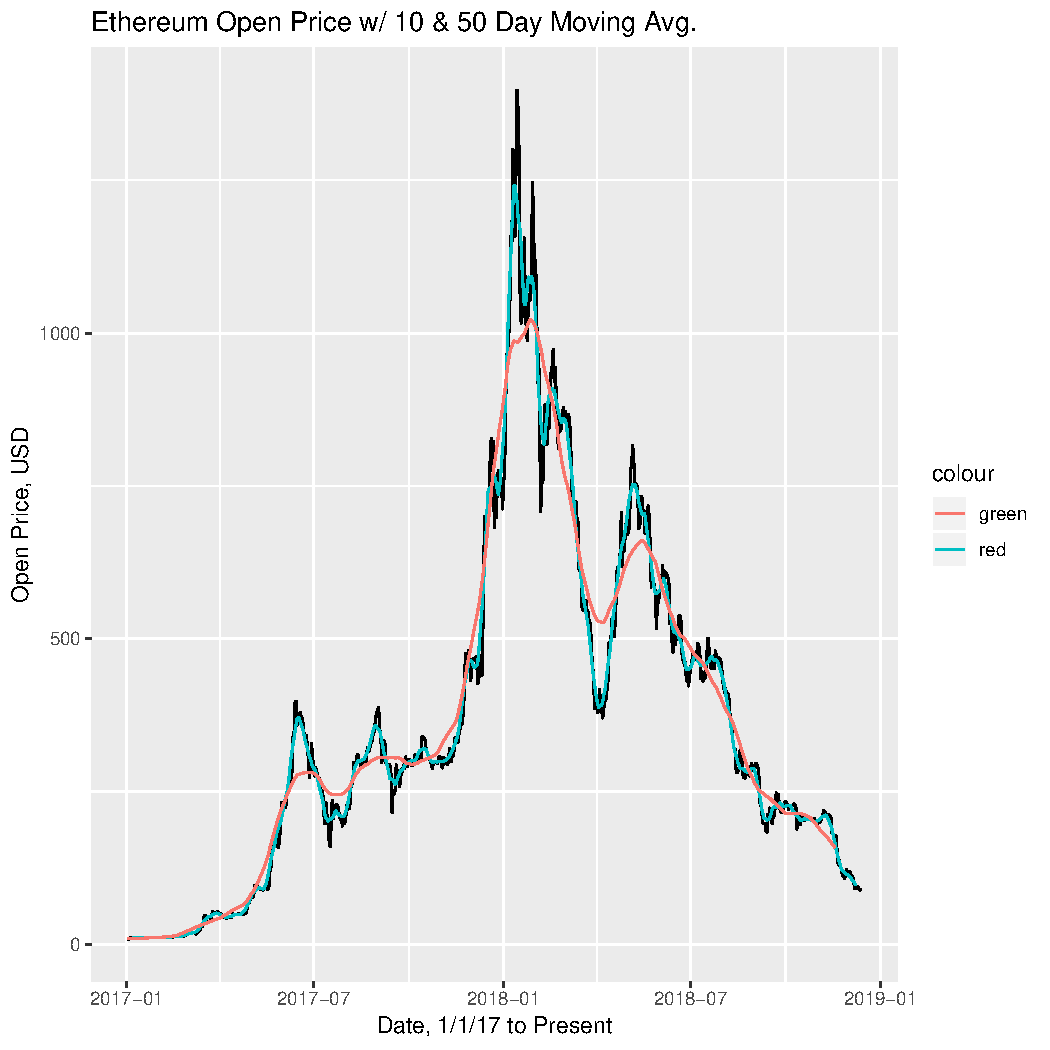
\includegraphics[width=.4\textwidth]{figure/open-1}}%<-NAME OF FIG 1
\qquad
\subfloat[Close]{%<-TITLE OF FIG2
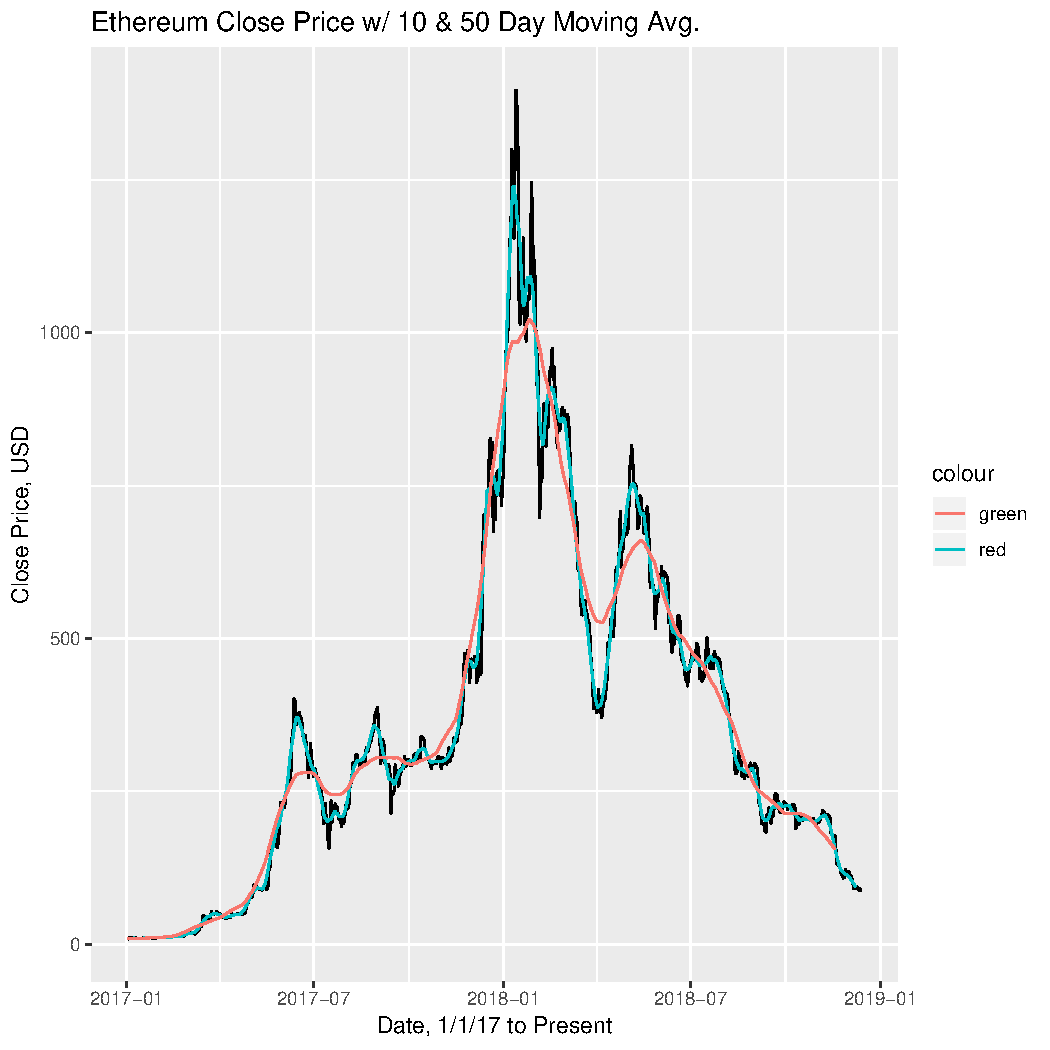
\includegraphics[width=.4\textwidth]{figure/close-1}}%<-NAME OF FIG 2
\end{center}
\end{figure}

\begin{figure}[ht]
\begin{center}
\subfloat[High]{%<-TITLE OF FIG3
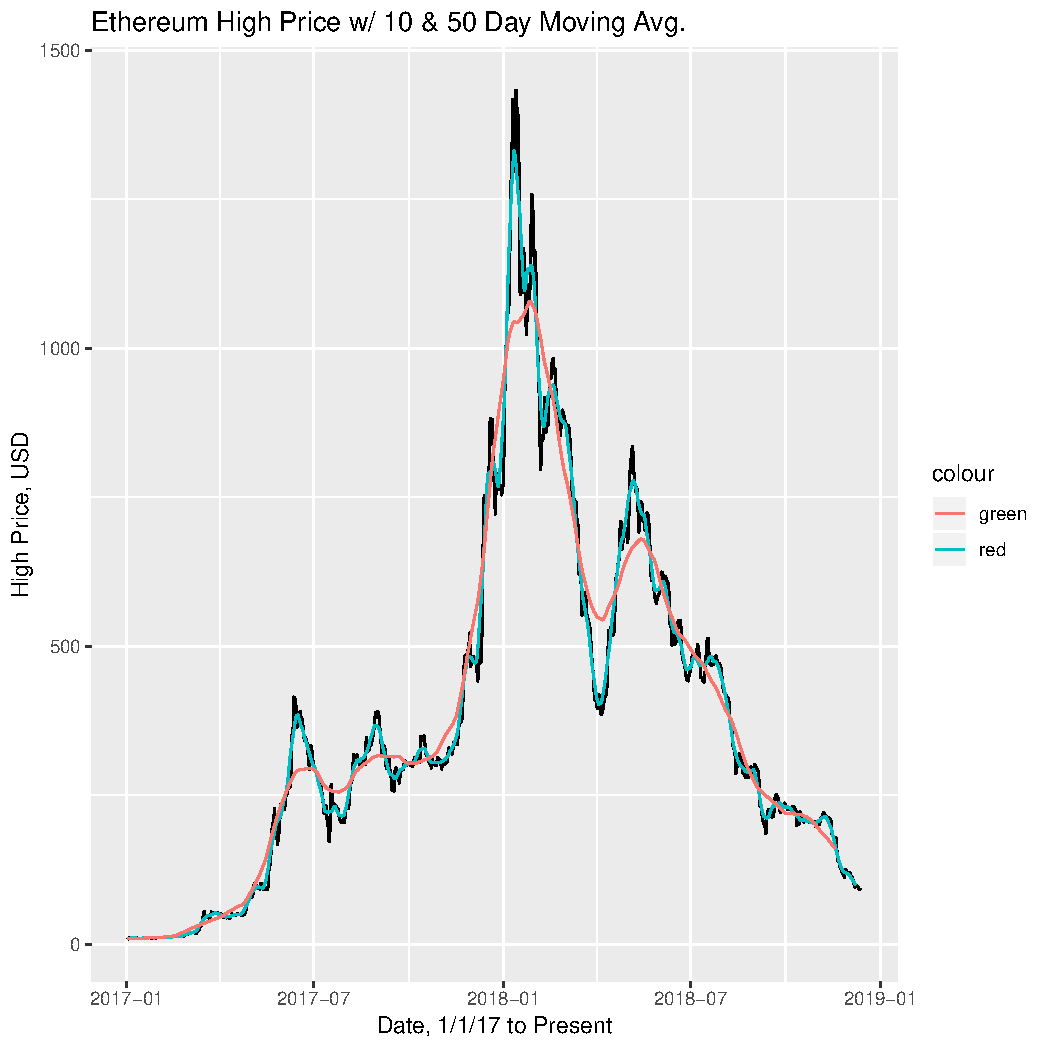
\includegraphics[width=.4\textwidth]{figure/high-1}}%<-NAME OF FIG3
\qquad
\subfloat[Low]{%<-TITLE OF FIG4
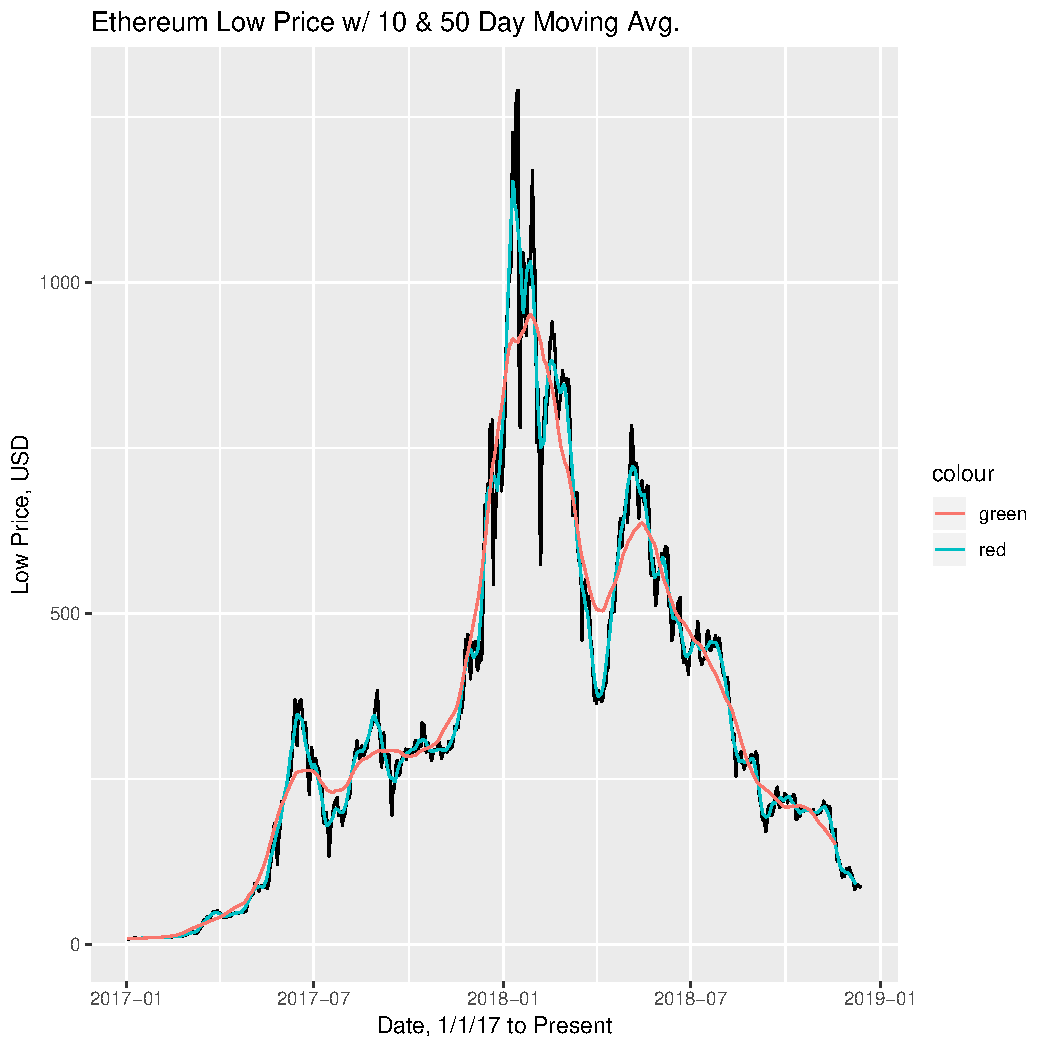
\includegraphics[width=.4\textwidth]{figure/low-1}}%<-NAME OF FIG4
\end{center}
\end{figure}

\subsection{Moving Forward w/ Model}
Now that the data has moving averages as well as past and previous values for open and close, it can be implemented in the form of a model. 
Yesterday's open, yesterday's close, today's open, today's close, historically the open and close of the next day, 10-day moving averages and 50-day moving averages can now be predictors used in the model, which could have a variety of useful outputs in trading. Namely, the difference between tomorrow's open and close values would be a useful prediction for traders, because it would indicate a predicted large shift in the market.

\section{Model Creation}
\subsection{Classification Models}
First make test and train sets.
The formula involving `closeNextBool` will predict whether tomorrow's close price wll be higher than today's close price.

\begin{knitrout}
\definecolor{shadecolor}{rgb}{0.969, 0.969, 0.969}\color{fgcolor}\begin{kframe}
\begin{alltt}
\hlstd{trainData} \hlkwb{<-} \hlkwd{sample_n}\hlstd{(dataRatio,}\hlkwd{nrow}\hlstd{(dataRatio)}\hlopt{*}\hlnum{0.8}\hlstd{)}
\hlstd{testData} \hlkwb{<-} \hlkwd{sample_n}\hlstd{(dataRatio,}\hlkwd{nrow}\hlstd{(dataRatio)}\hlopt{*}\hlnum{0.2}\hlstd{)}

\hlstd{formula} \hlkwb{<-} \hlkwd{as.formula}\hlstd{(}\hlstr{"closeNextBool~open*close*ma1*high*low*volume"}\hlstd{)}
\hlstd{lda.fit} \hlkwb{<-} \hlkwd{lda}\hlstd{(formula,testData)}
\hlstd{table}\hlkwb{<-}\hlkwd{table}\hlstd{(testData}\hlopt{$}\hlstd{closeNextBool,}
             \hlkwd{predict}\hlstd{(lda.fit,testData)}\hlopt{$}\hlstd{class)}
\hlstd{table}
\end{alltt}
\begin{verbatim}
##        
##         FALSE TRUE
##   FALSE   100   28
##   TRUE     37   80
\end{verbatim}
\end{kframe}
\end{knitrout}

Unfortunately, this model is not very accurate, showing an accuracy of
\begin{knitrout}
\definecolor{shadecolor}{rgb}{0.969, 0.969, 0.969}\color{fgcolor}\begin{kframe}
\begin{alltt}
\hlkwd{sum}\hlstd{(}\hlkwd{diag}\hlstd{(table))}\hlopt{/}\hlkwd{sum}\hlstd{(table)}\hlopt{*}\hlnum{100}
\end{alltt}
\begin{verbatim}
## [1] 73.46939
\end{verbatim}
\end{kframe}
\end{knitrout}

\subsection{Regression Models}
Recreate training and testing datasets.
\begin{knitrout}
\definecolor{shadecolor}{rgb}{0.969, 0.969, 0.969}\color{fgcolor}\begin{kframe}
\begin{alltt}
\hlstd{trainData} \hlkwb{<-} \hlkwd{sample_n}\hlstd{(dataRatio,}\hlkwd{nrow}\hlstd{(dataRatio)}\hlopt{*}\hlnum{0.8}\hlstd{)}
\hlstd{testData}\hlkwb{<-} \hlkwd{sample_n}\hlstd{(dataRatio,}\hlkwd{nrow}\hlstd{(dataRatio)}\hlopt{*}\hlnum{0.2}\hlstd{)}

\hlstd{formula} \hlkwb{<-} \hlkwd{as.formula}\hlstd{(}\hlstr{"closeNext~open*close*ma1*volume"}\hlstd{)}
\hlstd{glm.fit} \hlkwb{<-} \hlkwd{glm}\hlstd{(}\hlkwc{data}\hlstd{=trainData,}\hlkwc{formula}\hlstd{=formula)}
\hlkwd{mean}\hlstd{(}\hlkwd{predict}\hlstd{(glm.fit,testData)}\hlopt{/}\hlstd{testData}\hlopt{$}\hlstd{closeNext,}\hlkwc{na.rm}\hlstd{=}\hlnum{TRUE}\hlstd{)}
\end{alltt}
\begin{verbatim}
## [1] 0.9990149
\end{verbatim}
\end{kframe}
\end{knitrout}
\begin{center}
\begin{knitrout}
\definecolor{shadecolor}{rgb}{0.969, 0.969, 0.969}\color{fgcolor}\begin{kframe}
\begin{alltt}
\hlkwd{ggplot}\hlstd{(}\hlkwc{data}\hlstd{=}\hlkwd{data.frame}\hlstd{(}
    \hlkwc{prediction}\hlstd{=}\hlkwd{predict}\hlstd{(glm.fit,testData),}
    \hlkwc{value}\hlstd{=testData}\hlopt{$}\hlstd{closeNext))} \hlopt{+}
  \hlkwd{geom_point}\hlstd{(}\hlkwc{mapping} \hlstd{=} \hlkwd{aes}\hlstd{(}\hlkwc{x}\hlstd{=value,}\hlkwc{y}\hlstd{=prediction))}
\end{alltt}
\end{kframe}
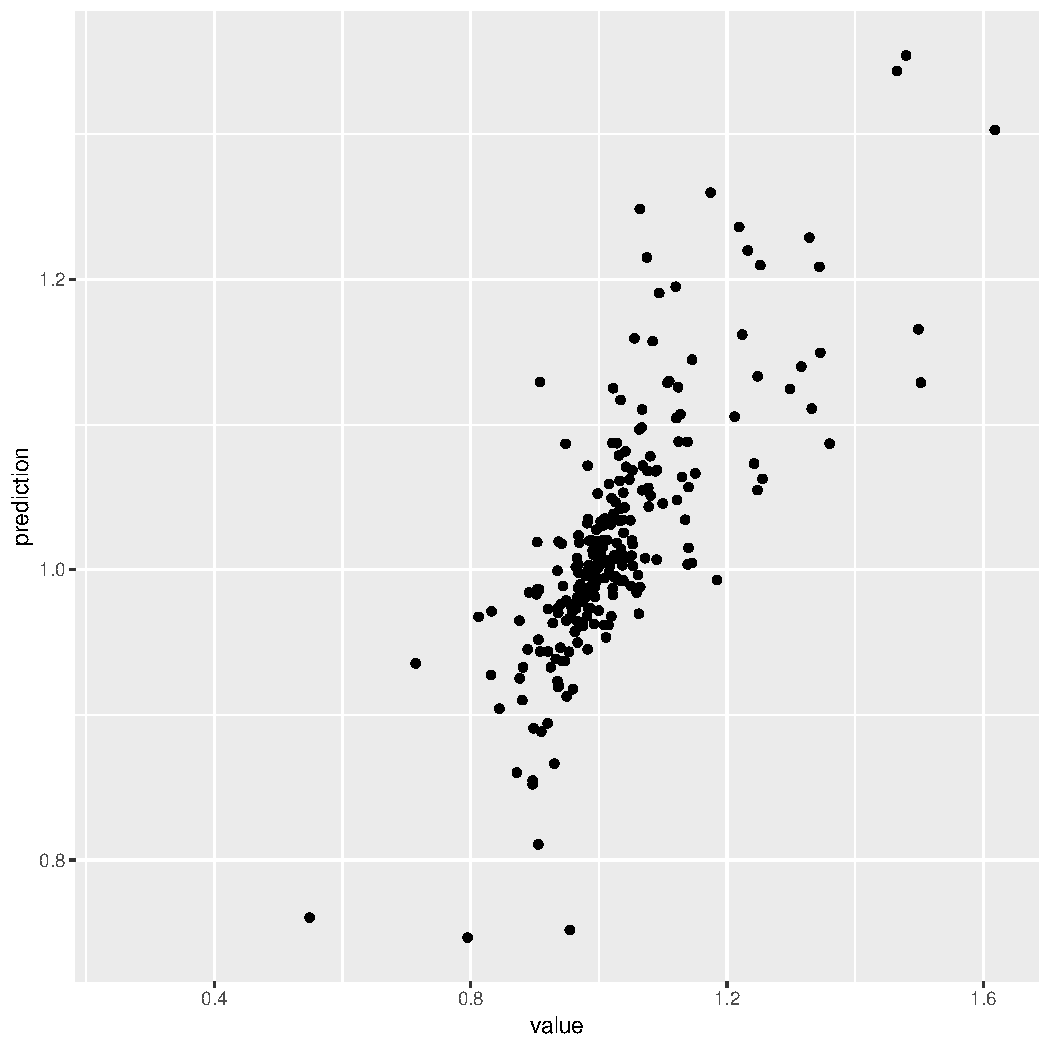
\includegraphics[width=3in,height=3in]{figure/unnamed-chunk-13-1} 

\end{knitrout}
\end{center}

\section{Model Evaluation}
\subsection{Visualizing Accuracy}
The following graph is a visual representation of the accuracy of the model, showing the percentage of predictions within the given percentage of the correct test data value. This was done using my function `glmVect()` in the file `modelData.R`. Note: The function `glmPlot()` in the same file performs the same computations, but saves a .png file of the plot, rather than returning a vector.
These functions were a majority of my work, and I believe these graphs are a great way to represent and visualize the accuracy of the model and to better understand the prediction vector output.

\begin{knitrout}
\definecolor{shadecolor}{rgb}{0.969, 0.969, 0.969}\color{fgcolor}\begin{kframe}
\begin{alltt}
\hlstd{formula} \hlkwb{<-} \hlkwd{as.formula}\hlstd{(}\hlstr{"closeNext~open*close*ma1*volume"}\hlstd{)}
\hlstd{percents} \hlkwb{<-} \hlkwd{seq}\hlstd{(}\hlnum{.1}\hlstd{,}\hlnum{10}\hlstd{,}\hlnum{.05}\hlstd{)}
\hlstd{result} \hlkwb{<-} \hlkwd{as.vector}\hlstd{(}
  \hlkwd{glmVect}\hlstd{(}\hlnum{1000}\hlstd{,}\hlnum{200}\hlstd{,percents,formula,}\hlkwc{forNum}\hlstd{=}\hlnum{100}\hlstd{,}\hlkwc{data}\hlstd{=dataRatio))}
\end{alltt}
\end{kframe}
\end{knitrout}
\begin{center}
\begin{knitrout}
\definecolor{shadecolor}{rgb}{0.969, 0.969, 0.969}\color{fgcolor}\begin{kframe}
\begin{alltt}
\hlkwd{ggplot}\hlstd{(}\hlkwc{data}\hlstd{=}\hlkwd{data.frame}\hlstd{(}\hlkwc{result}\hlstd{=result,}\hlkwc{value}\hlstd{=percents))} \hlopt{+}
  \hlkwd{geom_point}\hlstd{(}\hlkwc{mapping} \hlstd{=} \hlkwd{aes}\hlstd{(}\hlkwc{x}\hlstd{=value,}\hlkwc{y}\hlstd{=result))}
\end{alltt}
\end{kframe}
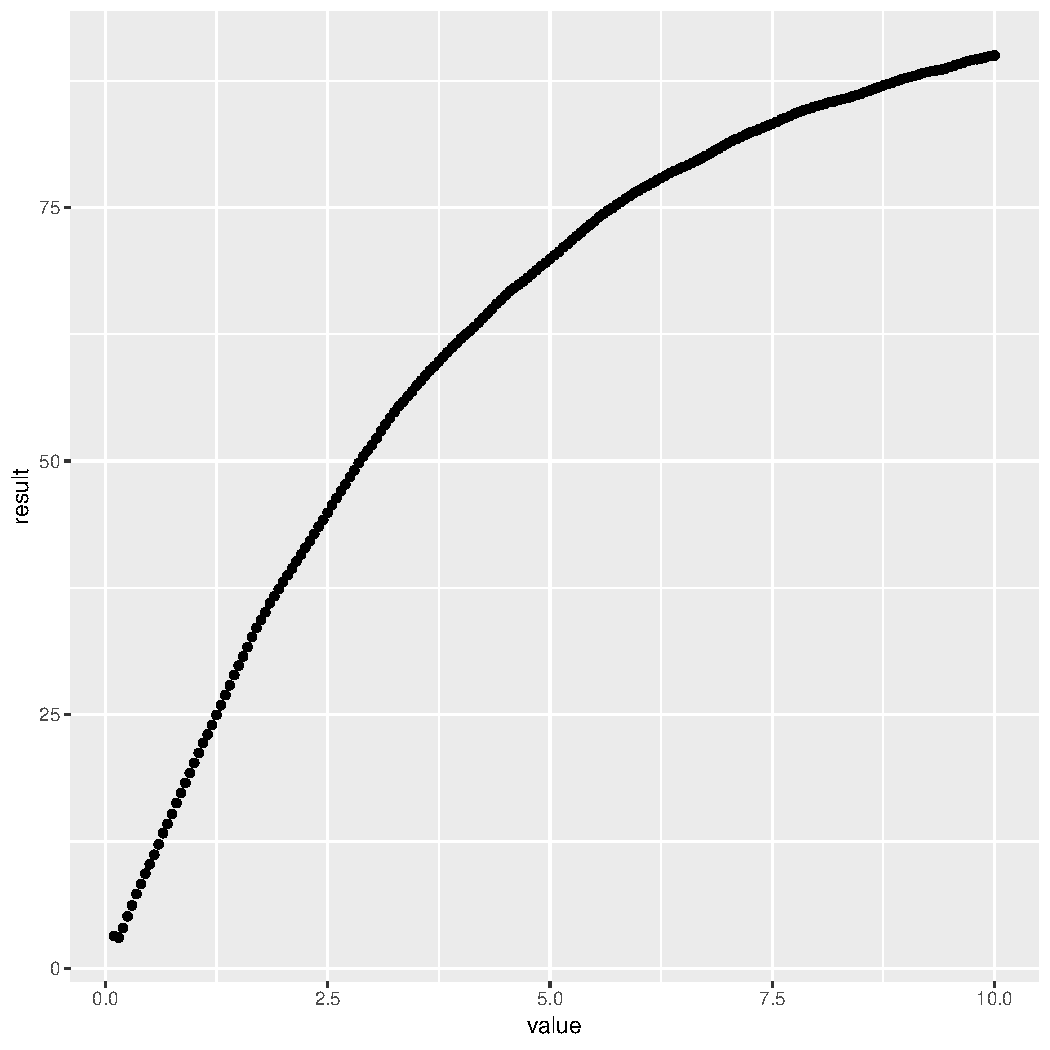
\includegraphics[width=3in,height=3in]{figure/unnamed-chunk-15-1} 

\end{knitrout}
\end{center}

The following is the same plot format as above, except using a compilation of ten different different formulas. In this case, the formulas are just each variable isolated.
\begin{knitrout}
\definecolor{shadecolor}{rgb}{0.969, 0.969, 0.969}\color{fgcolor}\begin{kframe}
\begin{alltt}
  \hlstd{formchar1}    \hlkwb{<-} \hlnum{0}
  \hlstd{formchar1[}\hlnum{1}\hlstd{]} \hlkwb{<-} \hlstr{"closeNext~open"}
  \hlstd{formchar1[}\hlnum{2}\hlstd{]} \hlkwb{<-} \hlstr{"closeNext~high"}
  \hlstd{formchar1[}\hlnum{3}\hlstd{]} \hlkwb{<-} \hlstr{"closeNext~low"}
  \hlstd{formchar1[}\hlnum{4}\hlstd{]} \hlkwb{<-} \hlstr{"closeNext~close"}
  \hlstd{formchar1[}\hlnum{5}\hlstd{]} \hlkwb{<-} \hlstr{"closeNext~volume"}
  \hlstd{formchar1[}\hlnum{6}\hlstd{]} \hlkwb{<-} \hlstr{"closeNext~market"}
  \hlstd{formchar1[}\hlnum{7}\hlstd{]} \hlkwb{<-} \hlstr{"closeNext~close_ratio"}
  \hlstd{formchar1[}\hlnum{8}\hlstd{]} \hlkwb{<-} \hlstr{"closeNext~spread"}
  \hlstd{formchar1[}\hlnum{9}\hlstd{]} \hlkwb{<-} \hlstr{"closeNext~ma1"}
  \hlstd{formchar1[}\hlnum{10}\hlstd{]}\hlkwb{<-} \hlstr{"closeNext~ma2"}

\hlstd{resultsdf} \hlkwb{<-} \hlkwd{formulaListGLM}\hlstd{(formchar1)}
\end{alltt}
\end{kframe}
\end{knitrout}

\begin{center}
\begin{knitrout}
\definecolor{shadecolor}{rgb}{0.969, 0.969, 0.969}\color{fgcolor}\begin{kframe}
\begin{alltt}
\hlkwd{ggplot}\hlstd{(}\hlkwc{data}\hlstd{=resultsdf)} \hlopt{+}
  \hlkwd{geom_point}\hlstd{(}\hlkwc{mapping} \hlstd{=} \hlkwd{aes}\hlstd{(}\hlkwc{x}\hlstd{=percents,}\hlkwc{y}\hlstd{=results,}\hlkwc{color}\hlstd{=formula))}
\end{alltt}
\end{kframe}
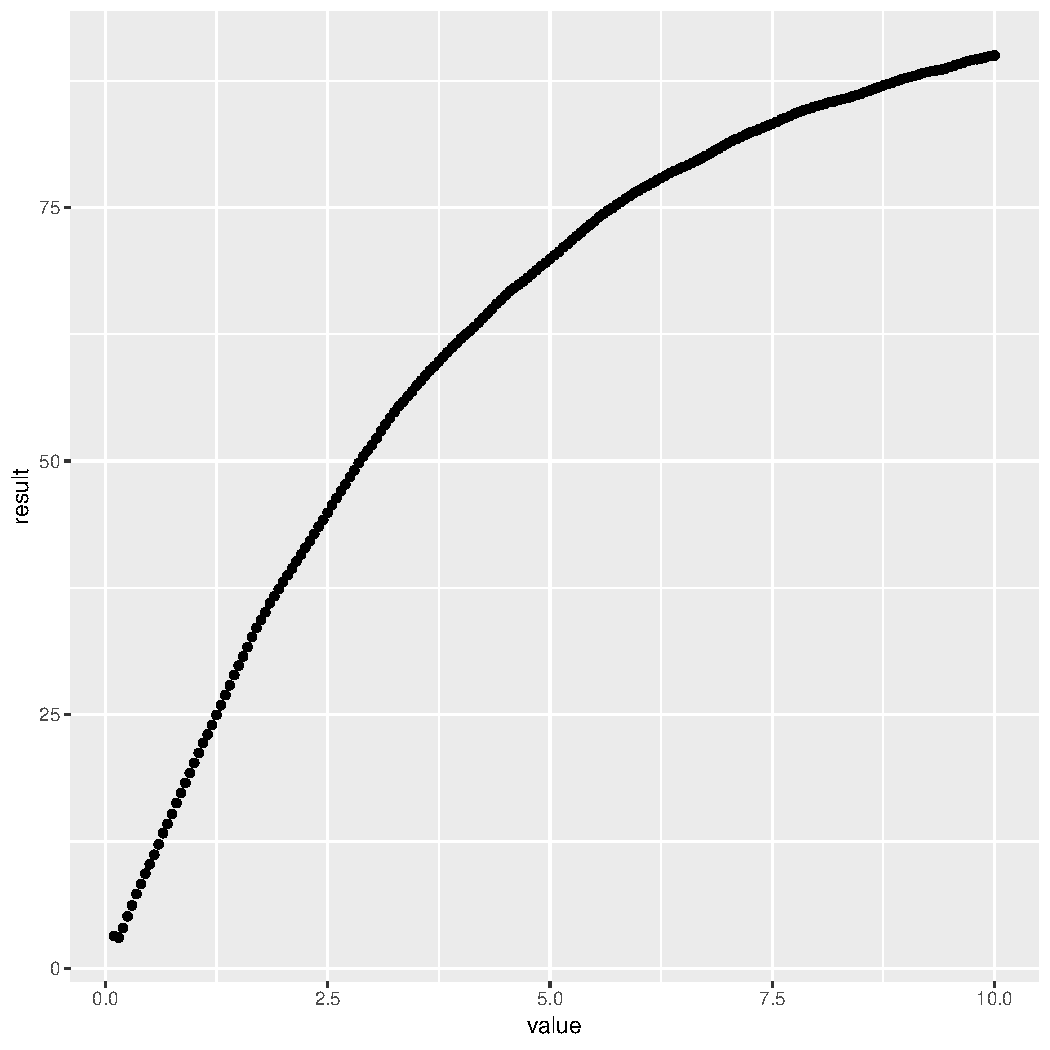
\includegraphics[width=3in,height=3in]{figure/unnamed-chunk-17-1} 

\end{knitrout}
\end{center}

\begin{knitrout}
\definecolor{shadecolor}{rgb}{0.969, 0.969, 0.969}\color{fgcolor}\begin{kframe}
\begin{alltt}
  \hlstd{formchar2}    \hlkwb{<-} \hlnum{0}
  \hlstd{formchar2[}\hlnum{1}\hlstd{]} \hlkwb{<-} \hlstr{"closeNext~open"}
  \hlstd{formchar2[}\hlnum{2}\hlstd{]} \hlkwb{<-} \hlstr{"closeNext~open*ma1"}
  \hlstd{formchar2[}\hlnum{3}\hlstd{]} \hlkwb{<-} \hlstr{"closeNext~open*ma1*close"}
  \hlstd{formchar2[}\hlnum{4}\hlstd{]} \hlkwb{<-} \hlstr{"closeNext~open*ma1*close*volume"}

  \hlstd{resultsdf} \hlkwb{<-} \hlkwd{formulaListGLM}\hlstd{(formchar2)}
\end{alltt}
\end{kframe}
\end{knitrout}

\begin{center}
\begin{knitrout}
\definecolor{shadecolor}{rgb}{0.969, 0.969, 0.969}\color{fgcolor}\begin{kframe}
\begin{alltt}
\hlkwd{ggplot}\hlstd{(}\hlkwc{data}\hlstd{=resultsdf)} \hlopt{+}
  \hlkwd{geom_point}\hlstd{(}\hlkwc{mapping} \hlstd{=} \hlkwd{aes}\hlstd{(}\hlkwc{x}\hlstd{=percents,}\hlkwc{y}\hlstd{=results,}\hlkwc{color}\hlstd{=formula))}
\end{alltt}
\end{kframe}
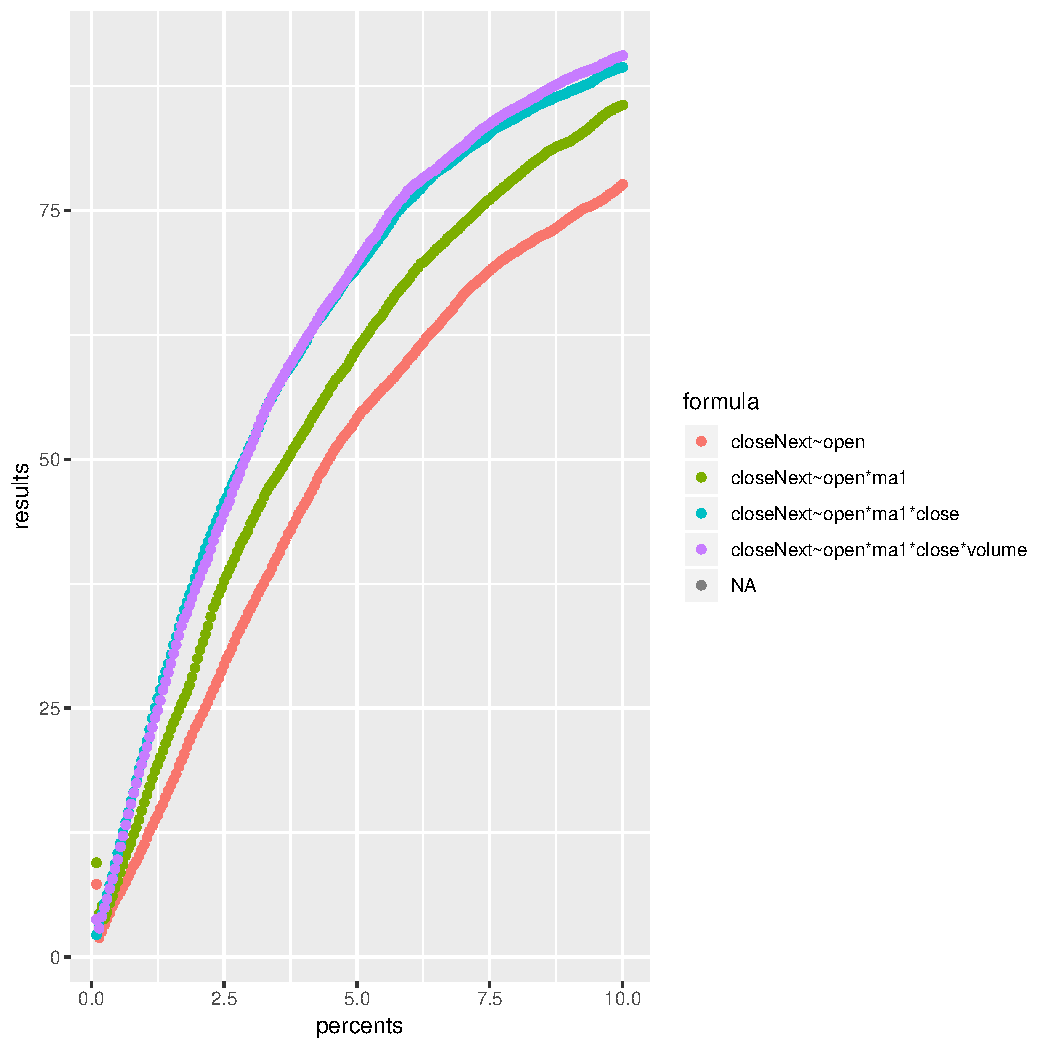
\includegraphics[width=3in,height=3in]{figure/unnamed-chunk-19-1} 

\end{knitrout}
\end{center}

\section{Conclusion}
In conclusion, simple analysis of historical data by day does not seem sufficient to predict the price of cryptocurrencies. This seems to be attributable to the tendency for manipulation of cryptocurrency, as well as the low volume in some markets that allows a select few "whales" to greatly influecne the market with large orders.\cite{liu2018risks} However, previous work that has been done has used social media reading in significantly more complicated models that had great success in crtpyocurrency price prediction using models similar to those in medical epidemic prediction.\cite{phillips2017predicting}\cite{kim2016predicting}

%=====================================================
\bibliographystyle{plain}
\bibliography{BIB}

%=====================================================
\end{document}
